\documentclass[handout]{beamer}
%\documentclass[]{beamer}
% ***************************************************************
% for handout, change only this...
%   \documentclass[twocolumn]{article}
%   \usepackage{beamerarticle}
%   \setlength{\textwidth}{7.5in}
%   \setlength{\textheight}{9.8in}
%   \setlength{\topmargin}{-1in}  
%   \setlength{\oddsidemargin}{-.52in}  
%   \setlength{\evensidemargin}{-.52in}  

%\usepackage{beamerprosper}
\usepackage{graphicx}
%\usepackage{psfrag, pstricks}
\usepackage{amsmath,amssymb,array,comment,eucal}
\newcommand{\e}{\mathbf{e}}
\renewcommand{\P}{\mathbf{P}}
\newcommand{\F}{\mathbf{F}}
\newcommand{\R}{\textsf{R}}
\newcommand{\mat}[1] {\mathbf{#1}}
%\newcommand{\ind}{\mathrel{\mathop{\sim}\limits^{\mathit{ind}}}}
%\newcommand{\iid}{\mathrel{\mathop{\sim}\limits^{\mathit{iid}}}}
\newcommand{\E}{\textsf{E}}
\newcommand{\SE}{\textsf{SE}}
\newcommand{\SSE}{\textsf{SSE}}
\newcommand{\RSS}{\textsf{RSS}}
\newcommand{\FSS}{\textsf{FSS}}
\renewcommand{\SS}{\textsf{SS}}
\newcommand{\MSE}{\textsf{MSE}}
\newcommand{\SSR}{\textsf{SSR}}
\newcommand{\Be}{\textsf{Beta}}
\newcommand{\St}{\textsf{St}}
%\newcommand{\C}{\textsf{C}}
\newcommand{\GDP}{\textsf{GDP}}
\newcommand{\NcSt}{\textsf{NcSt}}
\newcommand{\Bin}{\textsf{Bin}}
\newcommand{\NB}{\textsf{NegBin}}
\renewcommand{\NG}{\textsf{NG}}
\newcommand{\N}{\textsf{N}}
\newcommand{\Ber}{\textsf{Ber}}
\newcommand{\Poi}{\text{Poi}}
\newcommand{\Gam}{\textsf{Gamma}}
\newcommand{\BB}{\textsf{BB}}
\newcommand{\Gm}{\textsf{G}}
\newcommand{\Un}{\textsf{Unif}}
\newcommand{\Ex}{\textsf{Exp}}
\newcommand{\DE}{\textsf{DE}}
\newcommand{\tr}{\textsf{tr}}
\newcommand{\cF}{{\cal{F}}}
\newcommand{\cL}{{\cal{L}}}
\newcommand{\cI}{{\cal{I}}}
\newcommand{\cB}{{\cal{B}}}
\newcommand{\cP}{{\cal{P}}}
\newcommand{\bbR}{\mathbb{R}}
\newcommand{\bbN}{\mathbb{N}}
\newcommand{\pperp}{\mathrel{{\rlap{$\,\perp$}\perp\,\,}}}
\newcommand{\OFP}{(\Omega,\cF, \P)}
\newcommand{\eps}{\boldsymbol{\epsilon}}
\newcommand{\1}{\mathbf{1}_n}
\newcommand{\gap}{\vspace{8mm}}
\newcommand{\ind}{\mathrel{\mathop{\sim}\limits^{\rm ind}}}
\newcommand{\simiid}{\ensuremath{\mathrel{\mathop{\sim}\limits^{\rm
iid}}}}
\newcommand{\eqindis}{\ensuremath{\mathrel{\mathop{=}\limits^{\rm D}}}}
\newcommand{\iid}{\textit{i.i.d.}}
\newcommand{\SSZ}{S_{zz}}
\newcommand{\SZW}{S_{zw}}
\newcommand{\Var}{\textsf{Var}}
\newcommand{\corr}{\textsf{corr}}
\newcommand{\diag}{\textsf{diag}}
\newcommand{\var}{\textsf{var}}
\newcommand{\Cov}{\textsf{Cov}}
\newcommand{\Sam}{{\cal S}}
\def\H{\mathbf{H}}
\newcommand{\I}{\mathbf{I}}
\newcommand{\Y}{\mathbf{Y}}
\newcommand{\tY}{\tilde{\mathbf{Y}}}
\newcommand{\Yhat}{\hat{\mathbf{Y}}}
\newcommand{\Yobs}{\mathbf{Y}_{{\cal S}}}
\newcommand{\barYobs}{\bar{Y}_{{\cal S}}}
\newcommand{\barYmiss}{\bar{Y}_{{\cal S}^c}}
\def\bv{\mathbf{b}}
\def\X{\mathbf{X}}
\def\tX{\tilde{\mathbf{X}}}
\def\x{\mathbf{x}}
\def\xbar{\bar{\mathbf{x}}}
\def\Xbar{\bar{\mathbf{X}}}
\def\Xg{\mathbf{X}_{\boldsymbol{\gamma}}}
\def\Ybar{\bar{\Y}}
\def\ybar{\bar{y}}
\def\y{\mathbf{y}}
\def\Yf{\mathbf{Y_f}}
\def\W{\mathbf{W}}
\def\L{\mathbf{L}}
\def\w{\mathbf{w}}
\def\U{\mathbf{U}}
\def\V{\mathbf{V}}
\def\Q{\mathbf{Q}}
\def\Z{\mathbf{Z}}
\def\z{\mathbf{z}}
\def\v{\mathbf{v}}
\def\u{\mathbf{u}}

\def\zero{\mathbf{0}}
\def\one{\mathbf{1}}
\newcommand{\taub}{\boldsymbol{\tau}}
\newcommand{\betav}{\boldsymbol{\beta}}
\newcommand{\alphav}{\boldsymbol{\alpha}}
\newcommand{\A}{\mathbf{A}}
\def\a{\mathbf{a}}
\def\K{\mathbf{K}}
\newcommand{\B}{\mathbf{B}}
\def\b{\boldsymbol{\beta}}
\def\bhat{\hat{\boldsymbol{\beta}}}
\def\btilde{\tilde{\boldsymbol{\beta}}}
\def\tb{\tilde{\boldsymbol{\beta}}}
\def\bg{\boldsymbol{\beta_\gamma}}
\def\bgnot{\boldsymbol{\beta_{(-\gamma)}}}
\def\mub{\boldsymbol{\mu}}
\def\tmub{\tilde{\boldsymbol{\mu}}}
\def\muhat{\hat{\boldsymbol{\mu}}}
\def\t{\boldsymbol{\theta}}
\def\tk{\boldsymbol{\theta}_k}
\def\tj{\boldsymbol{\theta}_j}
\def\Mk{\boldsymbol{{\cal M}}_k}
\def\M{\boldsymbol{{\cal M}}}
\def\Mj{\boldsymbol{{\cal M}}_j}
\def\Mi{\boldsymbol{{\cal M}}_i}
\def\Mg{{\boldsymbol{{\cal M}_\gamma}}}
\def\Mnull{\boldsymbol{{\cal M}}_{N}}
\def\gMPM{\boldsymbol{\gamma}_{\text{MPM}}}
\def\gHPM{\boldsymbol{\gamma}_{\text{HPM}}}
\def\Mfull{\boldsymbol{{\cal M}}_{F}}
\def\tg{\boldsymbol{\theta}_{\boldsymbol{\gamma}}}
\def\g{\boldsymbol{\gamma}}
\def\eg{\boldsymbol{\eta}_{\boldsymbol{\gamma}}}
\def\G{\mathbf{G}}
\def\cM{\cal M}
\def\D{\Delta}
\def \shat{{\hat{\sigma}}^2}
\def\uv{\mathbf{u}}
\def\l {\lambda}
\def\d{\delta}
\def\Sigmab{\boldsymbol{\Sigma}}
\def\Lambdab{\boldsymbol{\Lambda}}
\def\lambdab{\boldsymbol{\lambda}}
\def\Mg{{\cal M}_\gamma}
\def\S{{\cal{S}}}
\def\qg{p_{\boldsymbol{\gamma}}}
\def\pg{p_{\boldsymbol{\gamma}}}
\def\t{\boldsymbol{\theta}}  
\def\T{\boldsymbol{\Theta}}  
\title{Model Choice}

\author{Hoff Chapter 9, Clyde \& George ``Model Uncertainty'' StatSci, Hoeting et al ``BMA'' StatSci} 
\date{\today}
%\Logo(-1.9,7.3){\includegraphics[width=.5in]{../eps/duke}}
% Optional: text to put in the bottom of each slide.
% By default, the title of the talk will be placed there.
%\slideCaption{\textit{October 28, 2005 }}

\begin{document}
% make the title slide
\maketitle
\begin{frame}\frametitle{Topics}
  \begin{itemize}
  \item Variable Selection / Model Choice
  \item Stepwise Methods
  \item Model Selection Criteria
  \item Model Averaging
  \end{itemize}
\end{frame}

\section{Variable Selection}
\begin{frame}\frametitle{Variable Selection}
  Reasons for reducing the number of variables in the model: \pause 
  \begin{itemize}
  \item  Philosophical \pause 
  \begin{itemize}
  \item Avoid the use of redundant variables (problems with
    interpretations) \pause 
  \item KISS \pause 
  \item Occam's Razor \pause 
  \end{itemize}
\item Practical  \pause 
  \begin{itemize}
  \item Inclusion of un-necessary terms yields less precise estimates,
    particularly if explanatory variables are highly correlated with
    each other \pause 
  \end{itemize}
\item it is too ``expensive'' to use all variables
  \end{itemize}
\end{frame}
\begin{frame}\frametitle{Variable Selection Procedures}
  \begin{itemize}
  \item Stepwise Regression:  Forward, Stepwise, Backward --
    add/delete variables until all t-statistics are significant (easy,
    but not recommended) \pause 
  \item Select variables with non-zero coefficients  from Lasso \pause 
  \item Select variables where shrinkage coefficient less than 0.5 \pause 
  \item Use a Model Selection Criterion to pick the ``best'' model  \pause 
    \begin{itemize}
    \item  R2 (picks largest model)  \pause 
      \item Adjusted R2  \pause 
      \item Mallow's Cp $C_p = (\text{SSE}/\hat{\sigma}_{Full}^2) + 2
        p_m - n $ \pause 
      \item AIC  (Akaike Information Criterion) proportional to Cp for
        linear models \pause 
      \item BIC(m)  (Bayes Information Criterion) $\hat{\sigma}_m^2 +
        \log(n) p_m$  \pause 
    \end{itemize}

  \end{itemize}
Trade off model complexity (number of coefficients $p_m$) with goodness of fit ( $\hat{\sigma}^2_m$)
\end{frame}

\begin{frame}\frametitle{Model Selection}
  Selection of a single model has the following problems \pause 
  \begin{itemize}
  \item When the criteria suggest that several models are equally
    good, what should we report?  Still pick only one model? \pause 
\item What do we report for our uncertainty after selecting a model?  \pause 
  \end{itemize}
Typical analysis ignores model uncertainty! \pause 
\vfill

Winner's Curse
\end{frame}

\begin{frame}\frametitle{Bayesian Model Choice}
  \begin{itemize}
  \item 
Models for the variable selection problem  are based on a subset of
  the $\X_1, \ldots \X_p$ variables  \pause 

\item Encode models with a  vector $\g = (\gamma_1, \ldots
  \gamma_p)$  where  $\gamma_j \in \{0,1\}$  
  is an indicator for whether variable $\X_j$ should be included in
  the model $\Mg$.  $\gamma_j = 0 \Leftrightarrow \beta_j
  = 0$  \pause 
\item Each value of $\g$ represents one of the $2^p$ models.
\pause 
\item Under model $\Mg$:
 $$\Y \mid \b, \sigma^2, \g \sim \N( \Xg \b_\gamma,
 \sigma^2 \I) $$
Where $\Xg$ is design matrix  using the columns in $\X$ where
 $\gamma_j = 1$ and $\b_{\g}$ is the subset of $\b$ that are non-zero.

\end{itemize}

\end{frame}

\begin{frame}\frametitle{Bayesian Model Averaging}
  Rather than use a single model, BMA uses all (or potentially a lot) models,
  but weights model predictions by their posterior probabilities
  (measure of how much each model is supported by the data) \pause 
  \begin{itemize}
  \item Posterior model probabilities
$$p(\M_j \mid \Y) = \frac{ p(\Y \mid \M_j)p(\M_j)}{\sum_jp(\Y \mid
  \M_j)p(\M_j)} $$ \pause 
Marginal likelihod of a model is proportional to 
$$ p(\Y \mid \Mg) = \iint p(\Y \mid \b_\gamma,
  \sigma^2)p(\b_\gamma \mid \g, \sigma^2)p(\sigma^2 \mid \g)
  d\b\, d\sigma^2$$\pause 
  \item Probability $\beta_j \ne 0$: $\sum_{\M_j:  \beta_j \ne 0}
    p(\M_j \mid \Y)$ (marginal inclusion probability) \pause 
  \item Predictions $$\hat{Y^*}| \Y  = \sum_j p(\M_j | \Y) \hat{Y}_{\M_j} $$
  \end{itemize}
\end{frame}


\begin{frame}\frametitle{Prior Distributions}
  \begin{itemize}
  \item Bayesian Model choice requires  proper prior distributions on
    parameters that are not common across models  \pause 
  \item Vague but proper priors may lead to paradoxes! \pause 
  \item Conjugate Normal-Gammas lead to closed form expressions for
  marginal likelihoods, Zellner's g-prior is the most popular. \pause 
  \end{itemize}
\end{frame}

\begin{frame}\frametitle{Zellner's g-prior}
  Centered model:  $$\Y = \1 \alpha + \X^c \b + \epsilon$$  
  where $\X^c$ is the centered design matrix where all variables have
  had their mean subtracted $\X^c = (\I - \P_{\1}) \X$ \pause 
\begin{itemize}
\item   $p(\alpha) \propto 1$ \pause 
\item  $p(\sigma^2) \propto 1/\sigma^2$  \pause 
\item  $\b_\gamma \mid \alpha, \sigma^2, \g \sim \N(0, g \sigma^2
  ({\X^c}^\prime \X^c)^{-1})$ \pause 
%\item  take $g=n$
\end{itemize}
which leads to marginal likelihood of $\Mg$ that is proportional
to $$ p(\Y \mid \Mg) = C (1 + g)^{\frac{n-p-1}{2}} ( 1 + g (1 -
 R^2_\gamma))^{- \frac{(n-1)}{2}}$$
where $R^2$ is the usual $R^2$ for model $\Mg$.
\pause 

Trade-off of model complexity versus goodness of fit

\bigskip
Lastly, assign prior distribution to space of models  (Uniform, or
Beta-binomial on model size)
\end{frame}

\begin{frame}[fragile]
\frametitle{USair Data}
\begin{verbatim}
library(BAS)
poll.bma = bas.lm(log(SO2) ~ temp + log(mgfirms) + 
                             log(popn) + wind + 
                             precip+ raindays, 
                  data=pollution, 
                  prior="g-prior", 
                  alpha=41,  # g = n
                  modelprior=uniform(),  # beta.binomial(1,6)
                  n.models=2^6, 
                  update=50, 
                  initprobs="Uniform")


par(mfrow=c(2,2))
plot(poll.bma, ask=F)
\end{verbatim}
\end{frame}
\begin{frame}\frametitle{Plots} 
  \centering 
  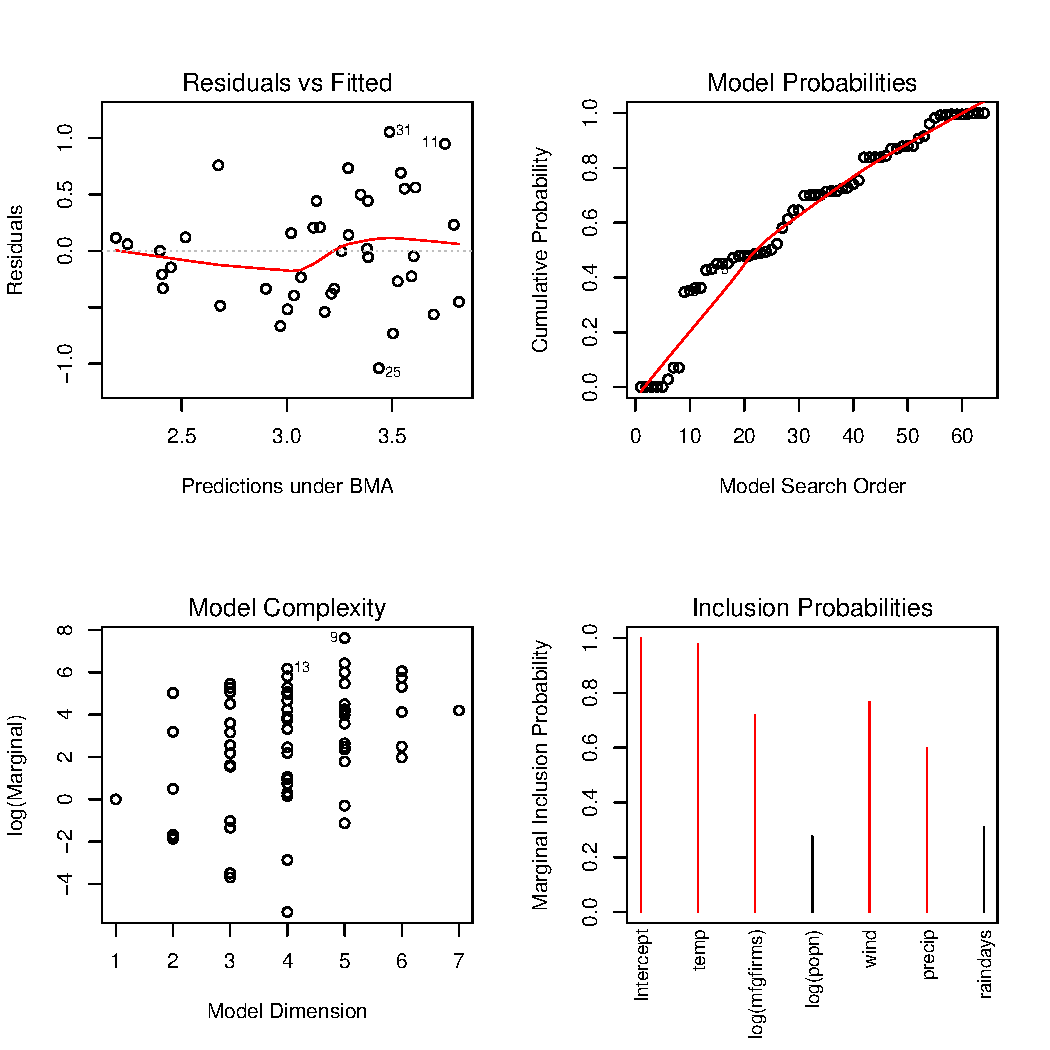
\includegraphics[height=3.5in]{poll-bma-sum}
\end{frame}

\begin{frame}\frametitle{Posterior Distribution  with Uniform Prior on Model Space}
image(poll.bma)
\centering
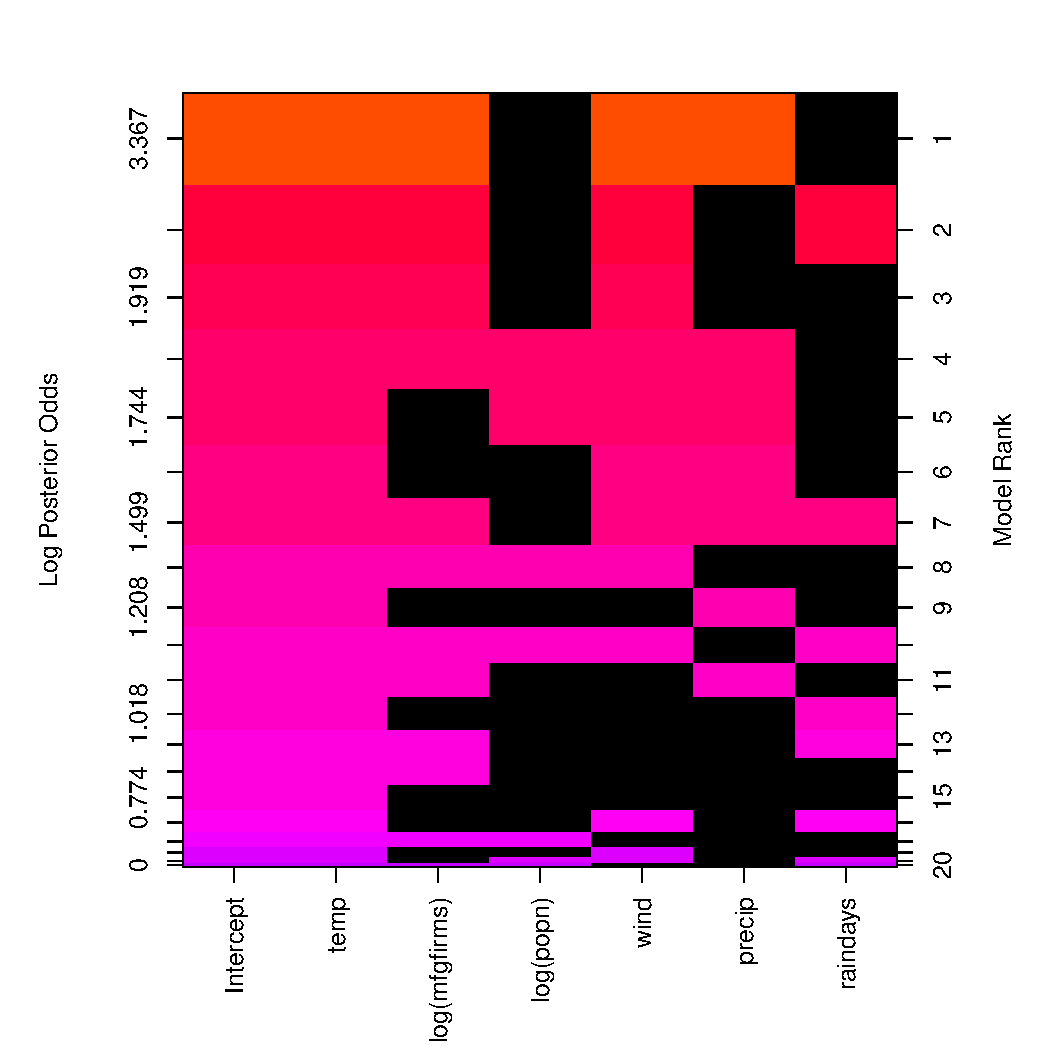
\includegraphics[height=3.5in]{poll-image}  
\end{frame}

\begin{frame}\frametitle{Posterior Distribution  with BB(1,p) Prior on Model Space}
image(poll-bb.bma)

\centering
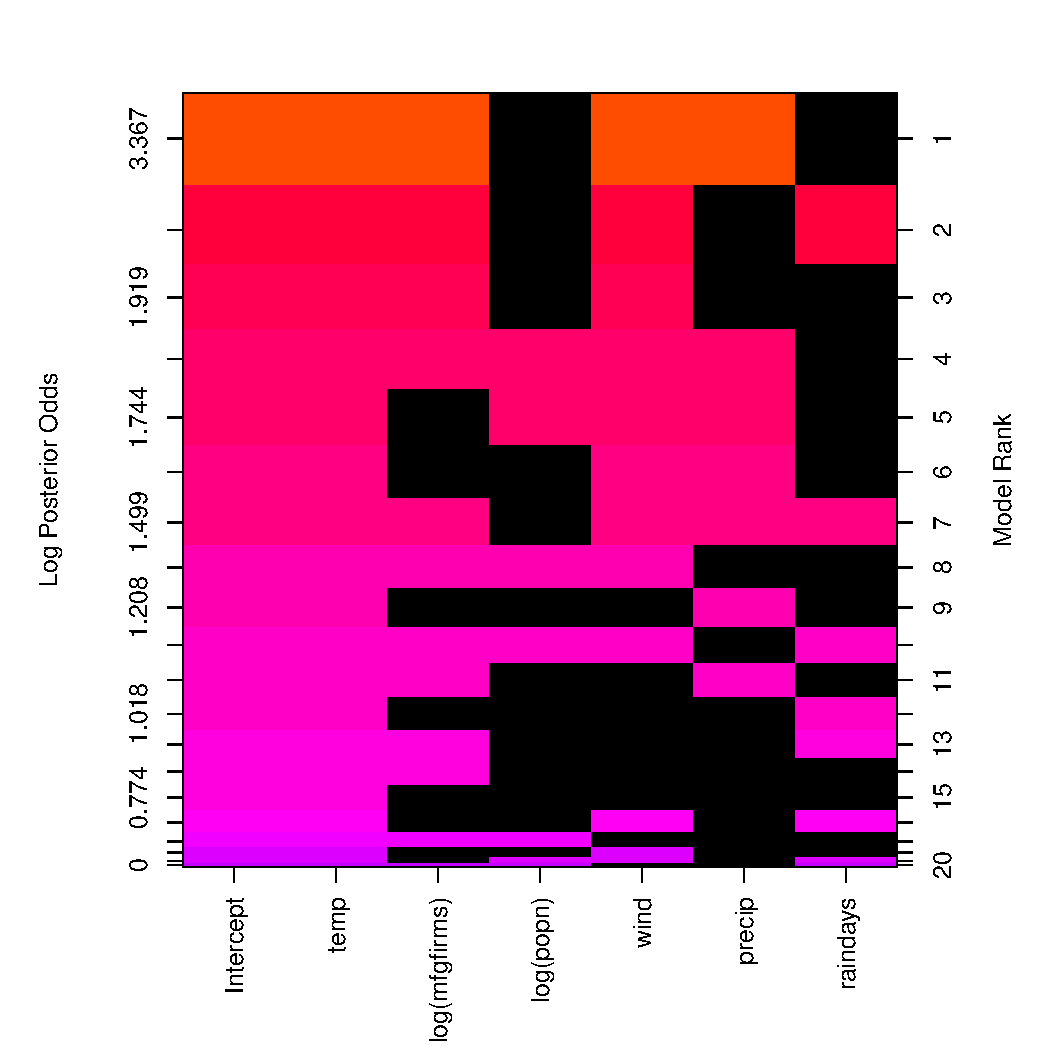
\includegraphics[height=3.5in]{poll-image}  
\end{frame}

\begin{frame}
\frametitle{Jeffreys Scale of Evidence}

$B = BF[H_o : B_a]$

\begin{tabular}{|r|l|} \hline \hline
Bayes Factor & Interpretation \\ \hline
$B \geq 1$ & $H_0$ supported \\
$1 > B \geq 10^{-\frac{1}{2}} $ & minimal evidence against $H_0$ \\
$ 10^{- \frac{1}{2}} > B  \geq 10^{-1}$ & substantial evidence against $H_0$ \\
$ 10^{-1} > B  \geq 10^{-2}$ & strong evidence against $H_0$ \\
$ 10^{-2} > B $ & decisive evidence against $H_0$ \\ \hline \hline
\end{tabular}

in context of testing one hypothesis with equal prior odds
\end{frame}


\begin{frame}[fragile]
\frametitle{Coefficients}
\begin{verbatim}
 beta = coef(poll.bma)
 par(mfrow=c(2,3));  plot(beta, subset=2:7,ask=F)
\end{verbatim}
\centering
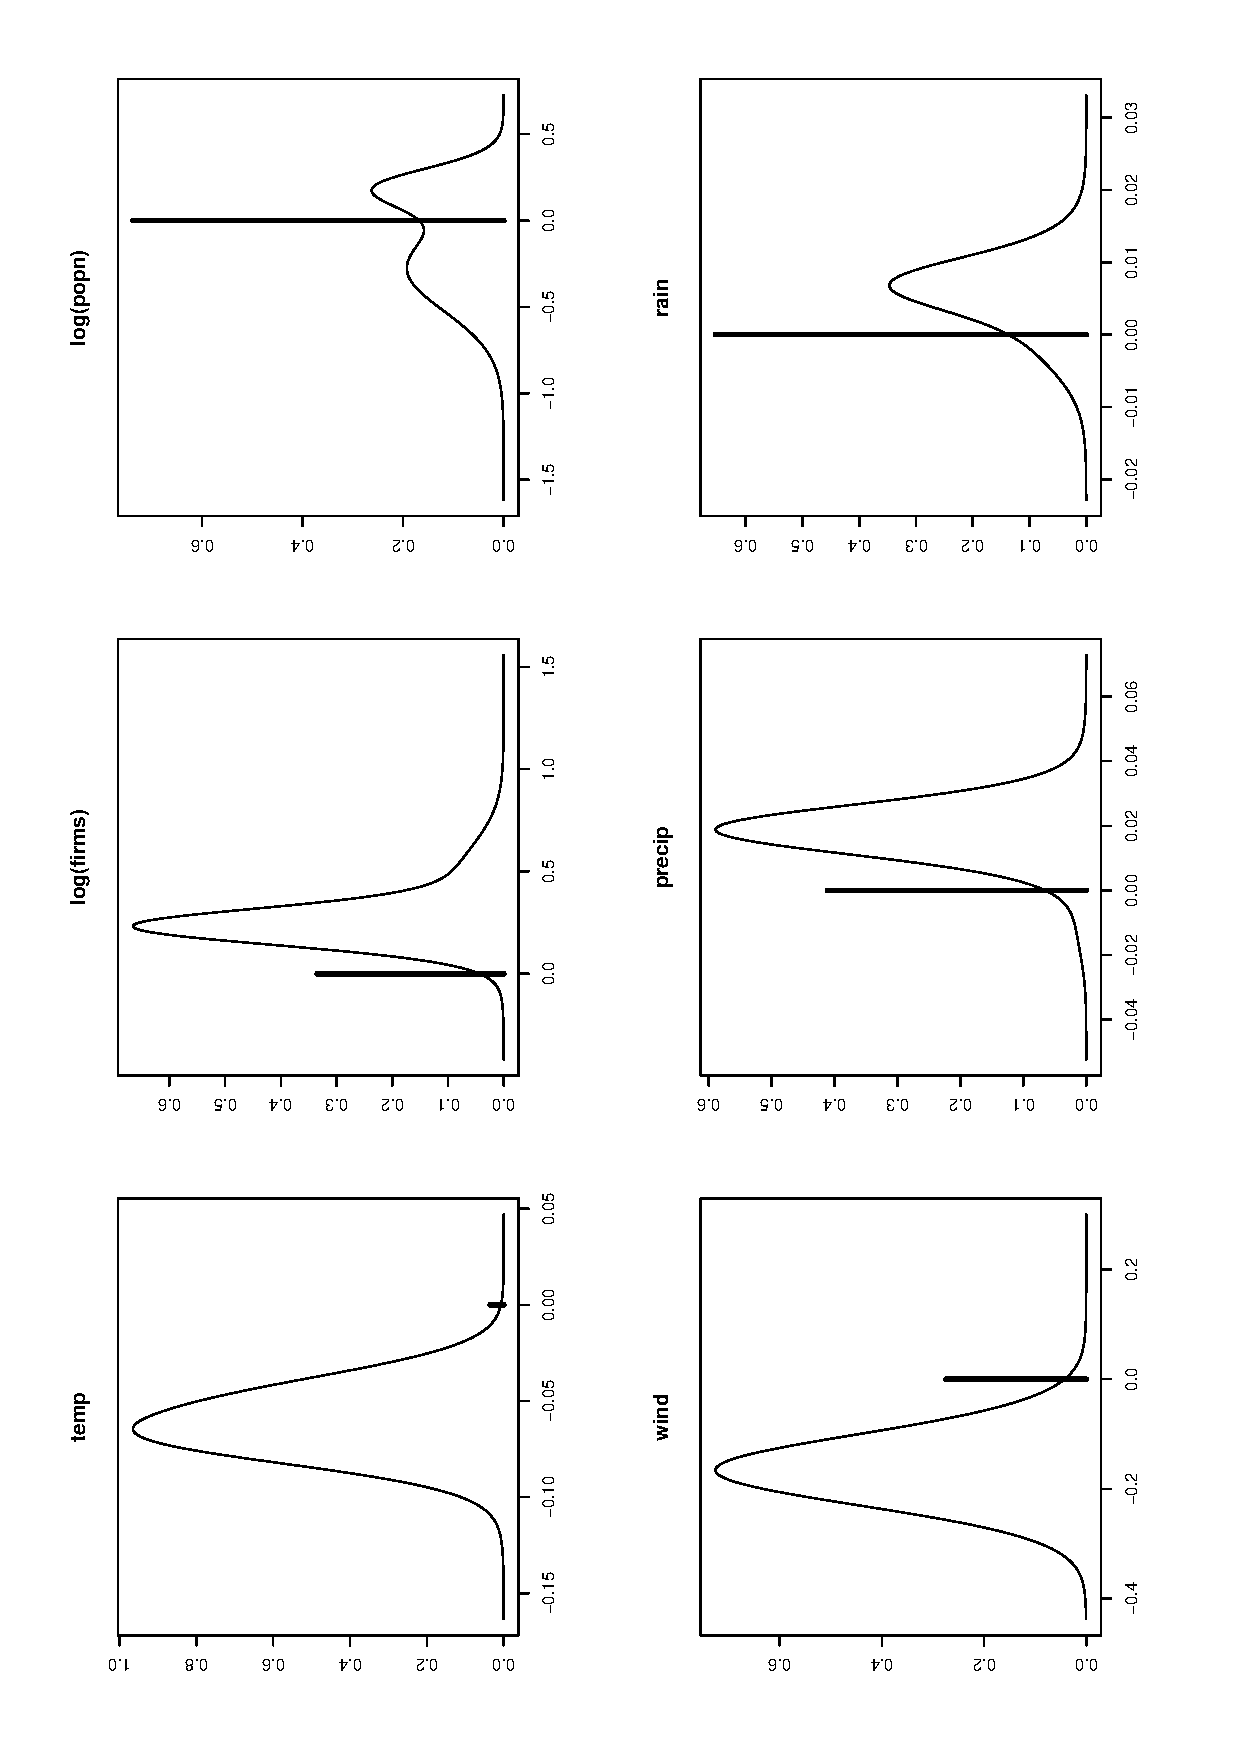
\includegraphics[height=3in]{poll-beta}  

\end{frame}

\begin{frame}
  \frametitle{Problem with g Prior}
The Bayes factor for comparing $\Mg$ to the null
model:
$$
 BF(\Mg : \M_0) =    (1 + g)^{(n - 1 - p_{\g})/2} (1 + g(1 - \R^2))^{(n-1)/2}
$$

\begin{itemize}
\item Let $g$ be a fixed constant and take $n$ fixed. 
\item Let $F = \frac{R_{\g}^2/\pg}{(1 - R_{\g}^2)/(n - 1 - \pg)}$
\item As $R^2_{\g} \to 1$, $F \to \infty$ LR test would reject $H_0$
\end{itemize}


usual $F$ statistic for  comparing model $\Mg$ to $\M_0$

\end{frame}

\section{Mortality}
\begin{frame}[fragile]
\frametitle{Mortality \& Pollution}
  \begin{itemize}
  \item Data from Statistical Sleuth 12.17 \pause 
  \item 60 cities \pause 
\item response Mortality \pause 
\item measures of HC, NOX, SO2 \pause 
\item Is pollution associated with mortality after adjusting for other
  socio-economic and meteorological factors? \pause 
\item 15 predictor variables implies $2^{15} = 32,768$ possible models
  \pause 
\item Use Zellner-Siow Cauchy prior  $1/g \sim  G(1/2, n/2)$
  \end{itemize}
\begin{verbatim}
mort.bma = bas.lm(MORTALITY ~ ., data=mortality,
                  prior="ZS-null", 
                  alpha=60,  n.models=2^15, 
                  update=100, initprobs="eplogp")
\end{verbatim}
\end{frame}

\begin{frame}\frametitle{Posterior Distributions}
  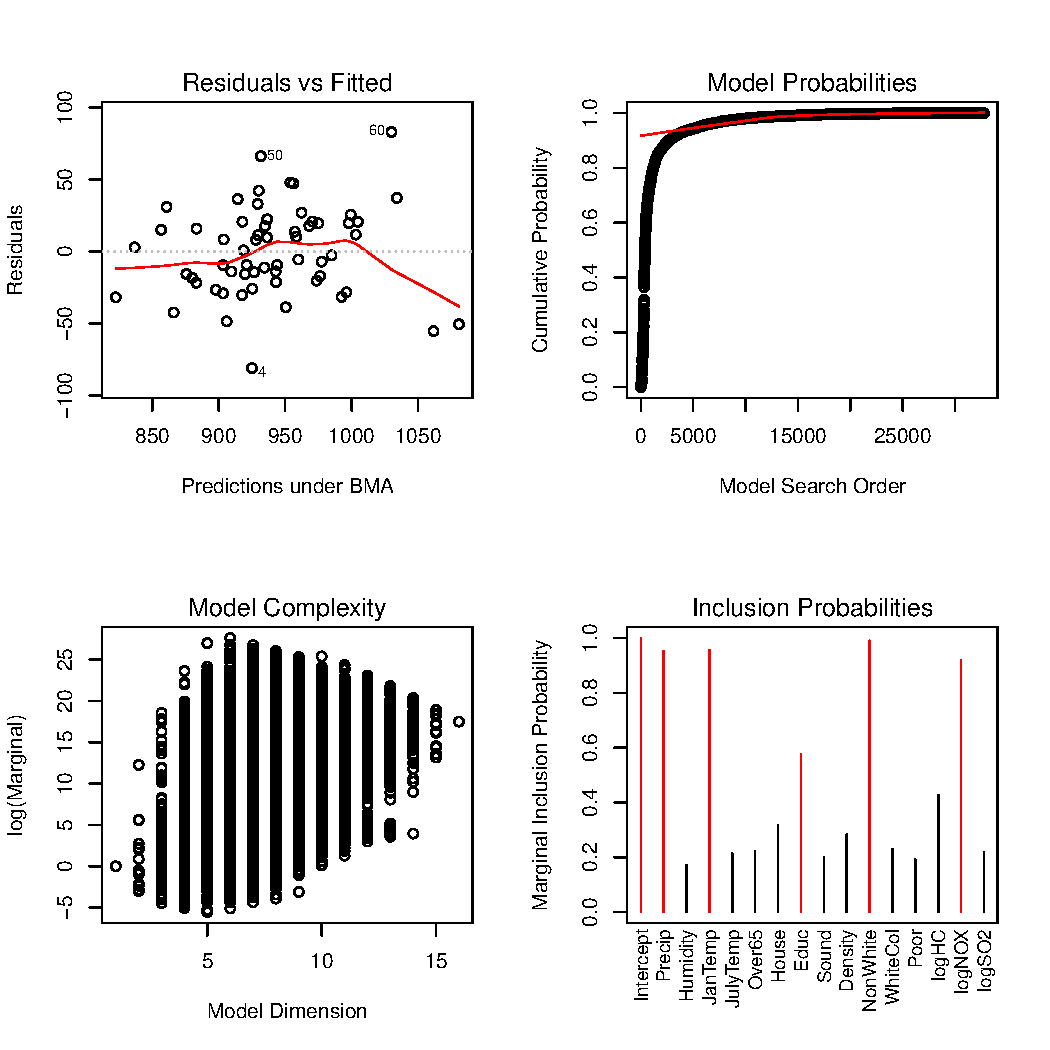
\includegraphics[height=3.5in]{mort-sum}
\end{frame}



\begin{frame}[fragile]
\frametitle{Posterior Probabilities}
  \begin{itemize}
  \item What is the probability that there is no pollution effect? \pause 
\item Sum posterior model probabilities over all models that include
  at least one pollution variable \pause 
\begin{verbatim}
> which.mat = list2matrix.which(mort.bma,1:(2^15))
> poll.in = (which.mat[, 14:16] %*% rep(1, 3)) > 0
> sum(poll.in * mort.bma$postprob)
[1] 0.9889641
\end{verbatim}\pause 
\item Posterior probability no effect is $0.011$ \pause 
\item Odds that there is an effect  $(1 - .011)/(.011) = 89.9$ \pause 
\item Prior Odds $7 = (1 - .5^3)/.5^3$ \pause 
\item Bayes Factor for a pollution effect $ 89.9/7= 12.8$ \pause 
\item Bayes Factor for NOXEffect  based on marginal inclusion probability
  $0.917/(1 - 0.917) = 11.0$ \pause  
\item Marginal inclusion probability for logHC =  0.4271; BF = 0.75
\item Marginal inclusion probability for logSO2 = 0.2189; BF = 0.28
\end{itemize}
Note Bayes Factors are not additive!
\end{frame}
\begin{frame}\frametitle{Model Space}
  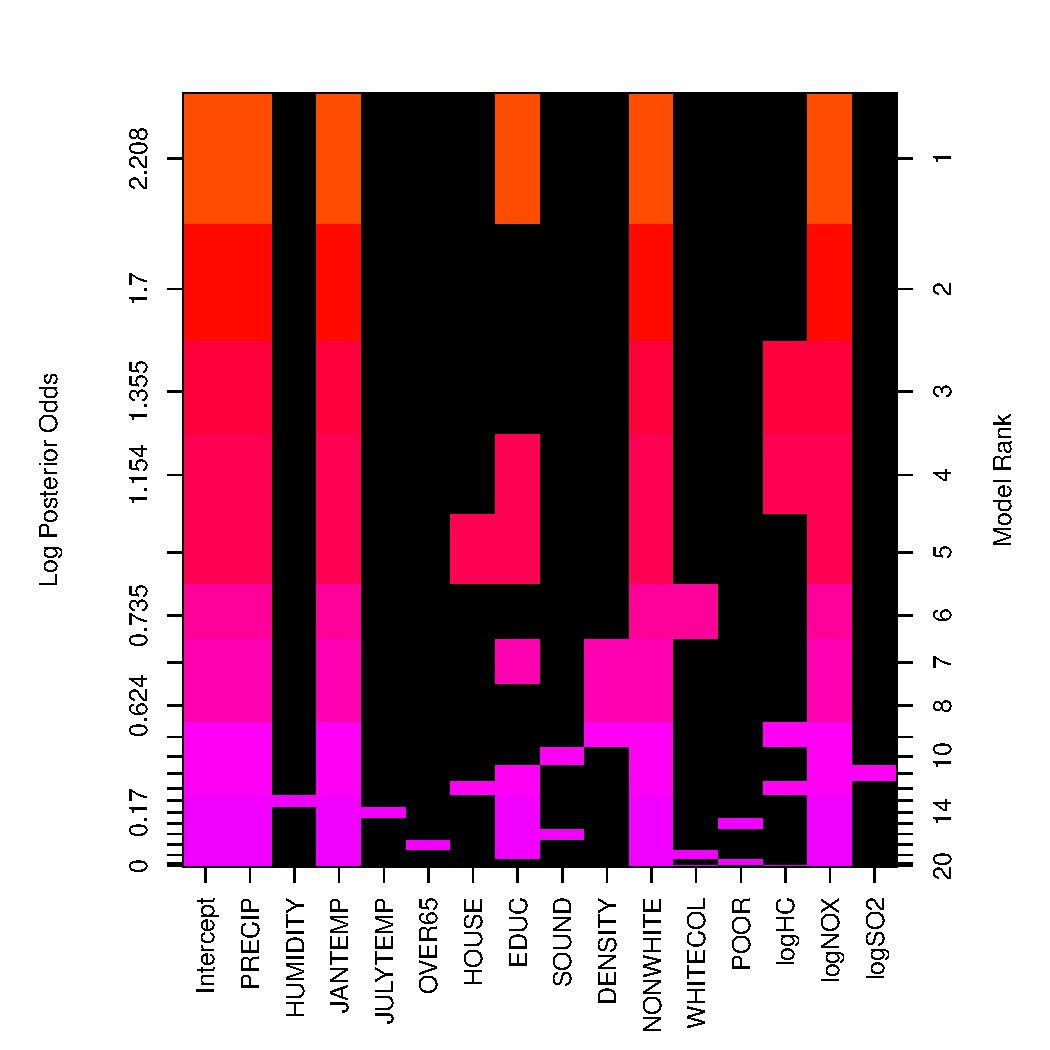
\includegraphics[height=3.5in]{mort-image}
\end{frame}
\begin{frame}\frametitle{Coefficients}
  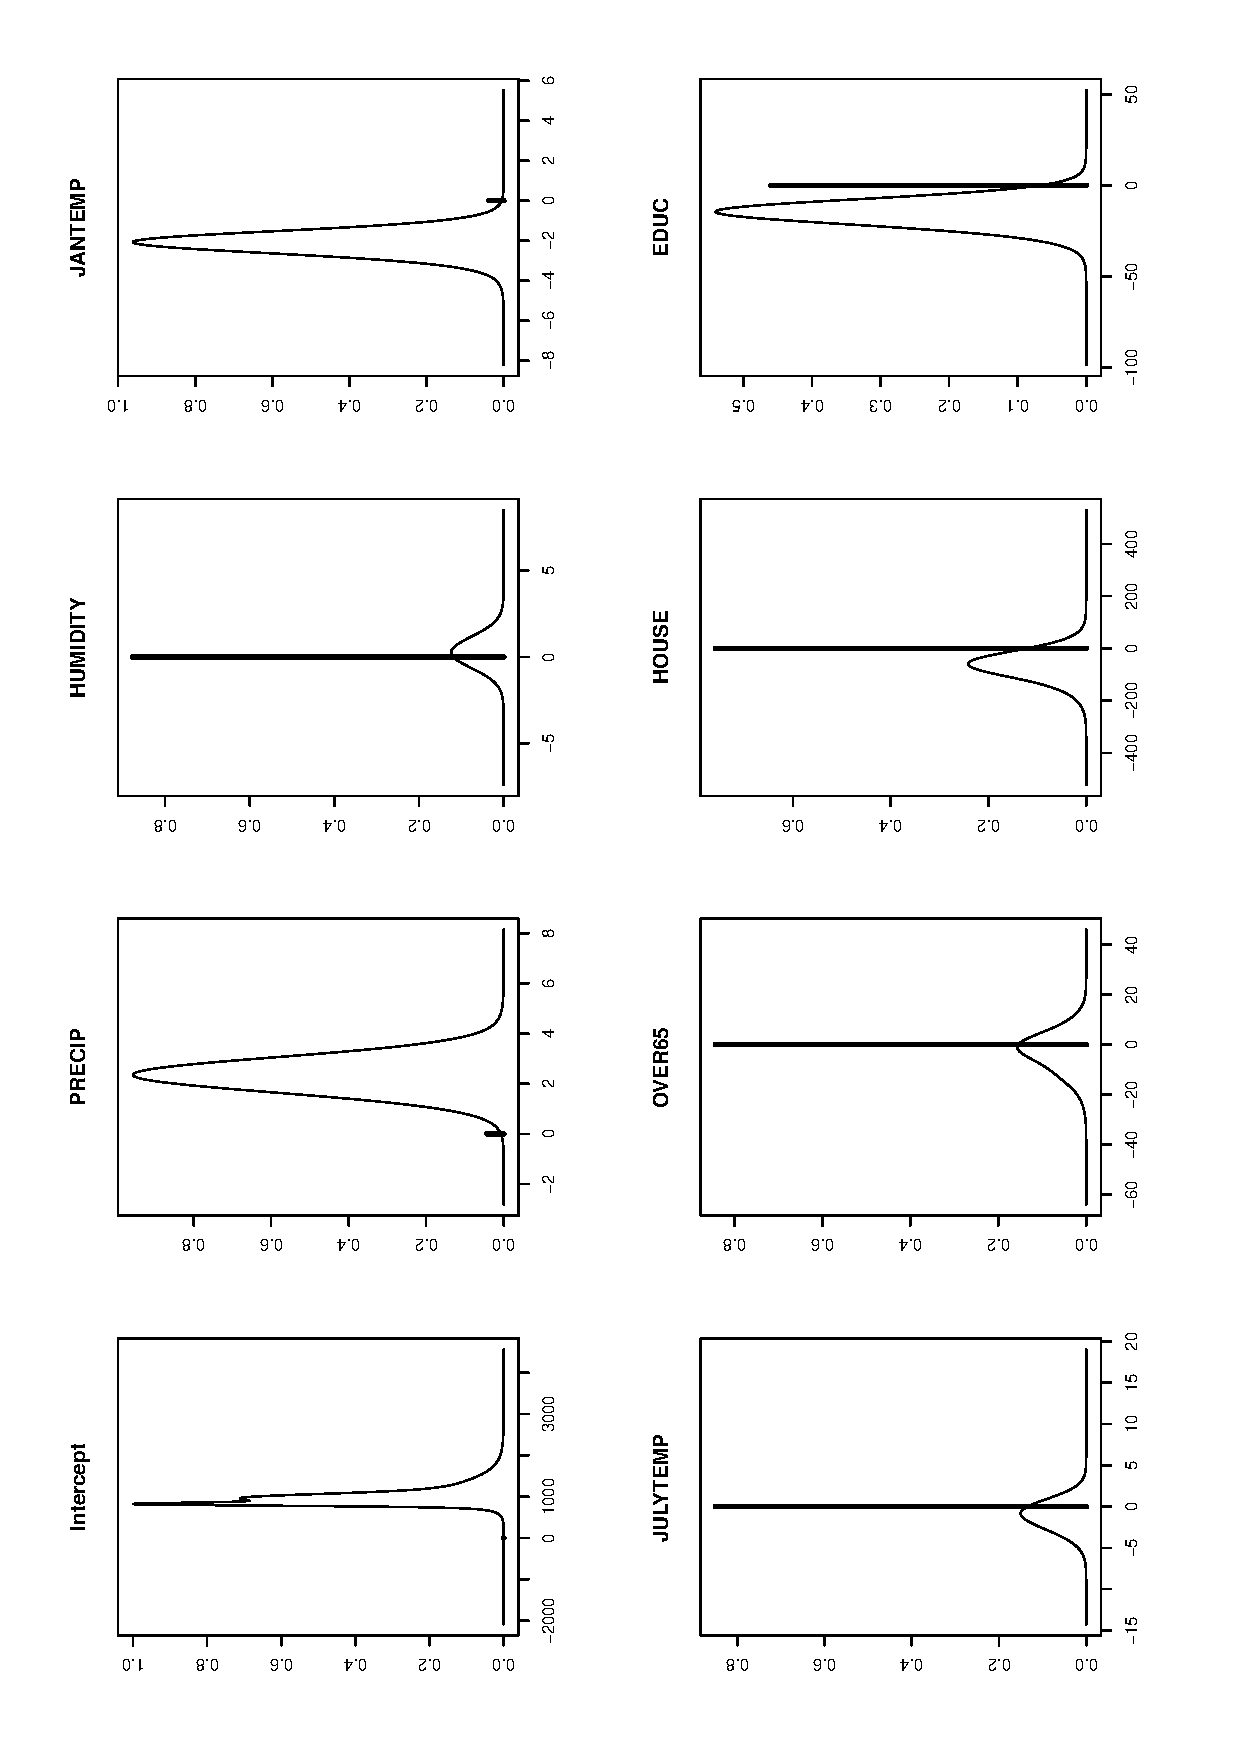
\includegraphics[height=3.5in]{mort-beta1}
\end{frame}

\begin{frame}\frametitle{Coefficients}
  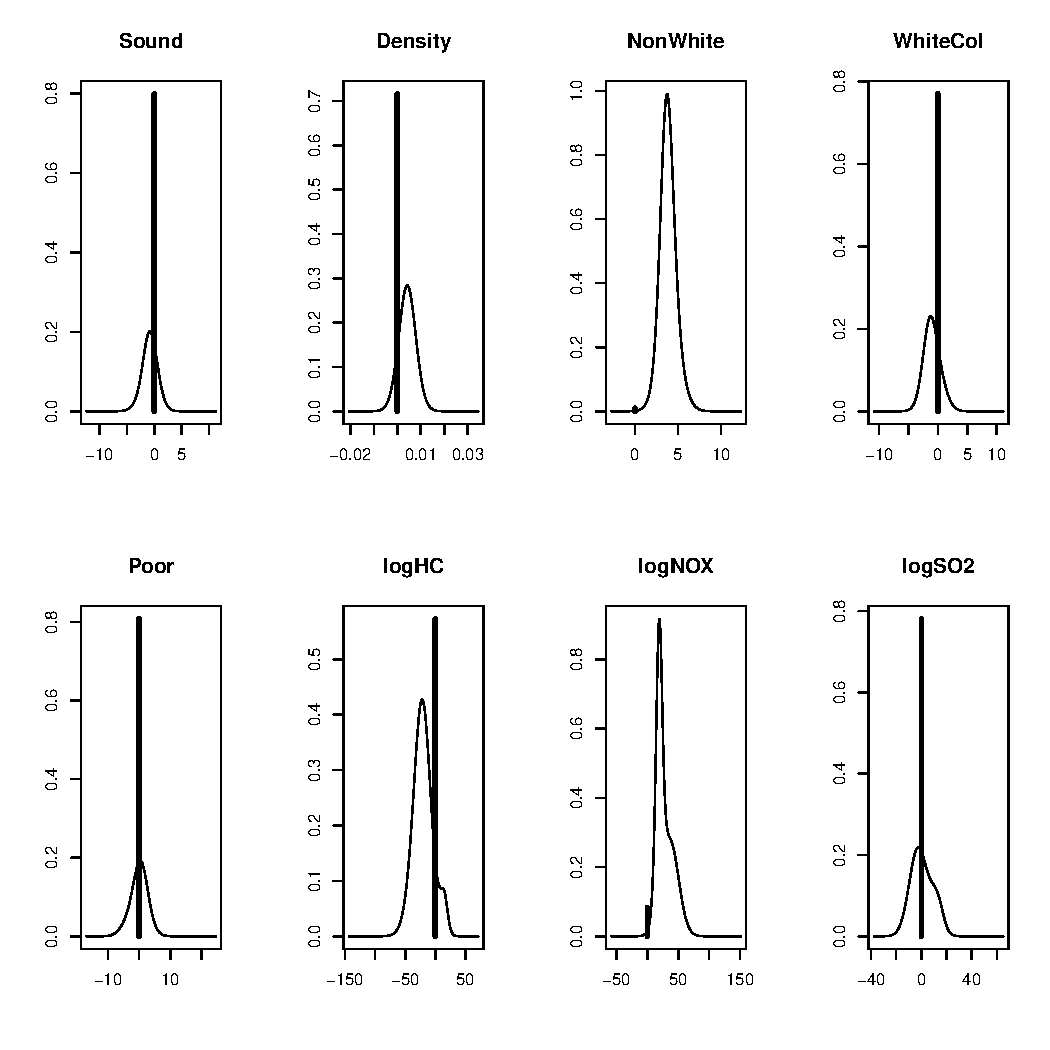
\includegraphics[height=3.5in]{mort-beta2}
\end{frame}

\begin{frame}
  \frametitle{Effect Estimation}
  \begin{itemize}
  \item  Coefficients in each model are adjusted for other variables
    in the model
\item OLS:  leave out a predictor with a non-zero coefficient then
  estimates are biased!
\item Model Selection in the presence of high correlation, may leave
  out "redundant" variables; 
\item improved MSE for prediction (Bias-variance tradeoff)
\item Bayes is biased anyway so should we care?
\item What is meaning of $\sum_{\g} \beta_{j \g} \gamma_j P(\Mg \mid \Y)$
  \end{itemize}
  Problem with confounding!  Need to change prior?

\end{frame}



\begin{frame}\frametitle{ Other Problems}


  \begin{itemize}
  \item Computational \pause 
  if $p > 35$  enumeration is difficult \pause 
  \begin{itemize}
  \item Gibbs sampler or Random-Walk algorithm on $\g$ \pause 
  \item poor convergence/mixing with high correlations \pause 
  \item Metropolis Hastings algorithms more flexibility \pause 
  \item "Stochastic Search" (no guarantee samples represent posterior) \pause 
  \item in BMA all variables are included, but coefficients are 
   shrunk to 0; alternative is to use Shrinkage methods \pause 
  \end{itemize}
\item Prior Choice: Choice of prior distributions on $\b$ and on $\g$ \pause 
\end{itemize}

\bigskip Model averaging versus Model Selection  -- what are objectives?


\end{frame}
\end{document}
